\documentclass[a4paper,12pt]{article}
\usepackage[slovene]{babel}
\usepackage[utf8]{inputenc}
\usepackage{multicol}
\usepackage{fullpage}
\usepackage{guitar}
\usepackage{titlesec}
\usepackage{graphicx}
\setcounter{secnumdepth}{-1} 
\usepackage[absolute]{textpos}
\titleformat{\chapter}{\large\bfseries}{\thesection}{1em}{}
\titleformat{\section}{\Large\bfseries}{\thesection}{1em}{}
\titleformat{\subsection}{\large\bfseries}{\thesection}{1em}{}

\begin{document}
\pagenumbering{Roman}
\begin{titlepage}
\begin{textblock*}{297mm}(-6mm,-0mm)
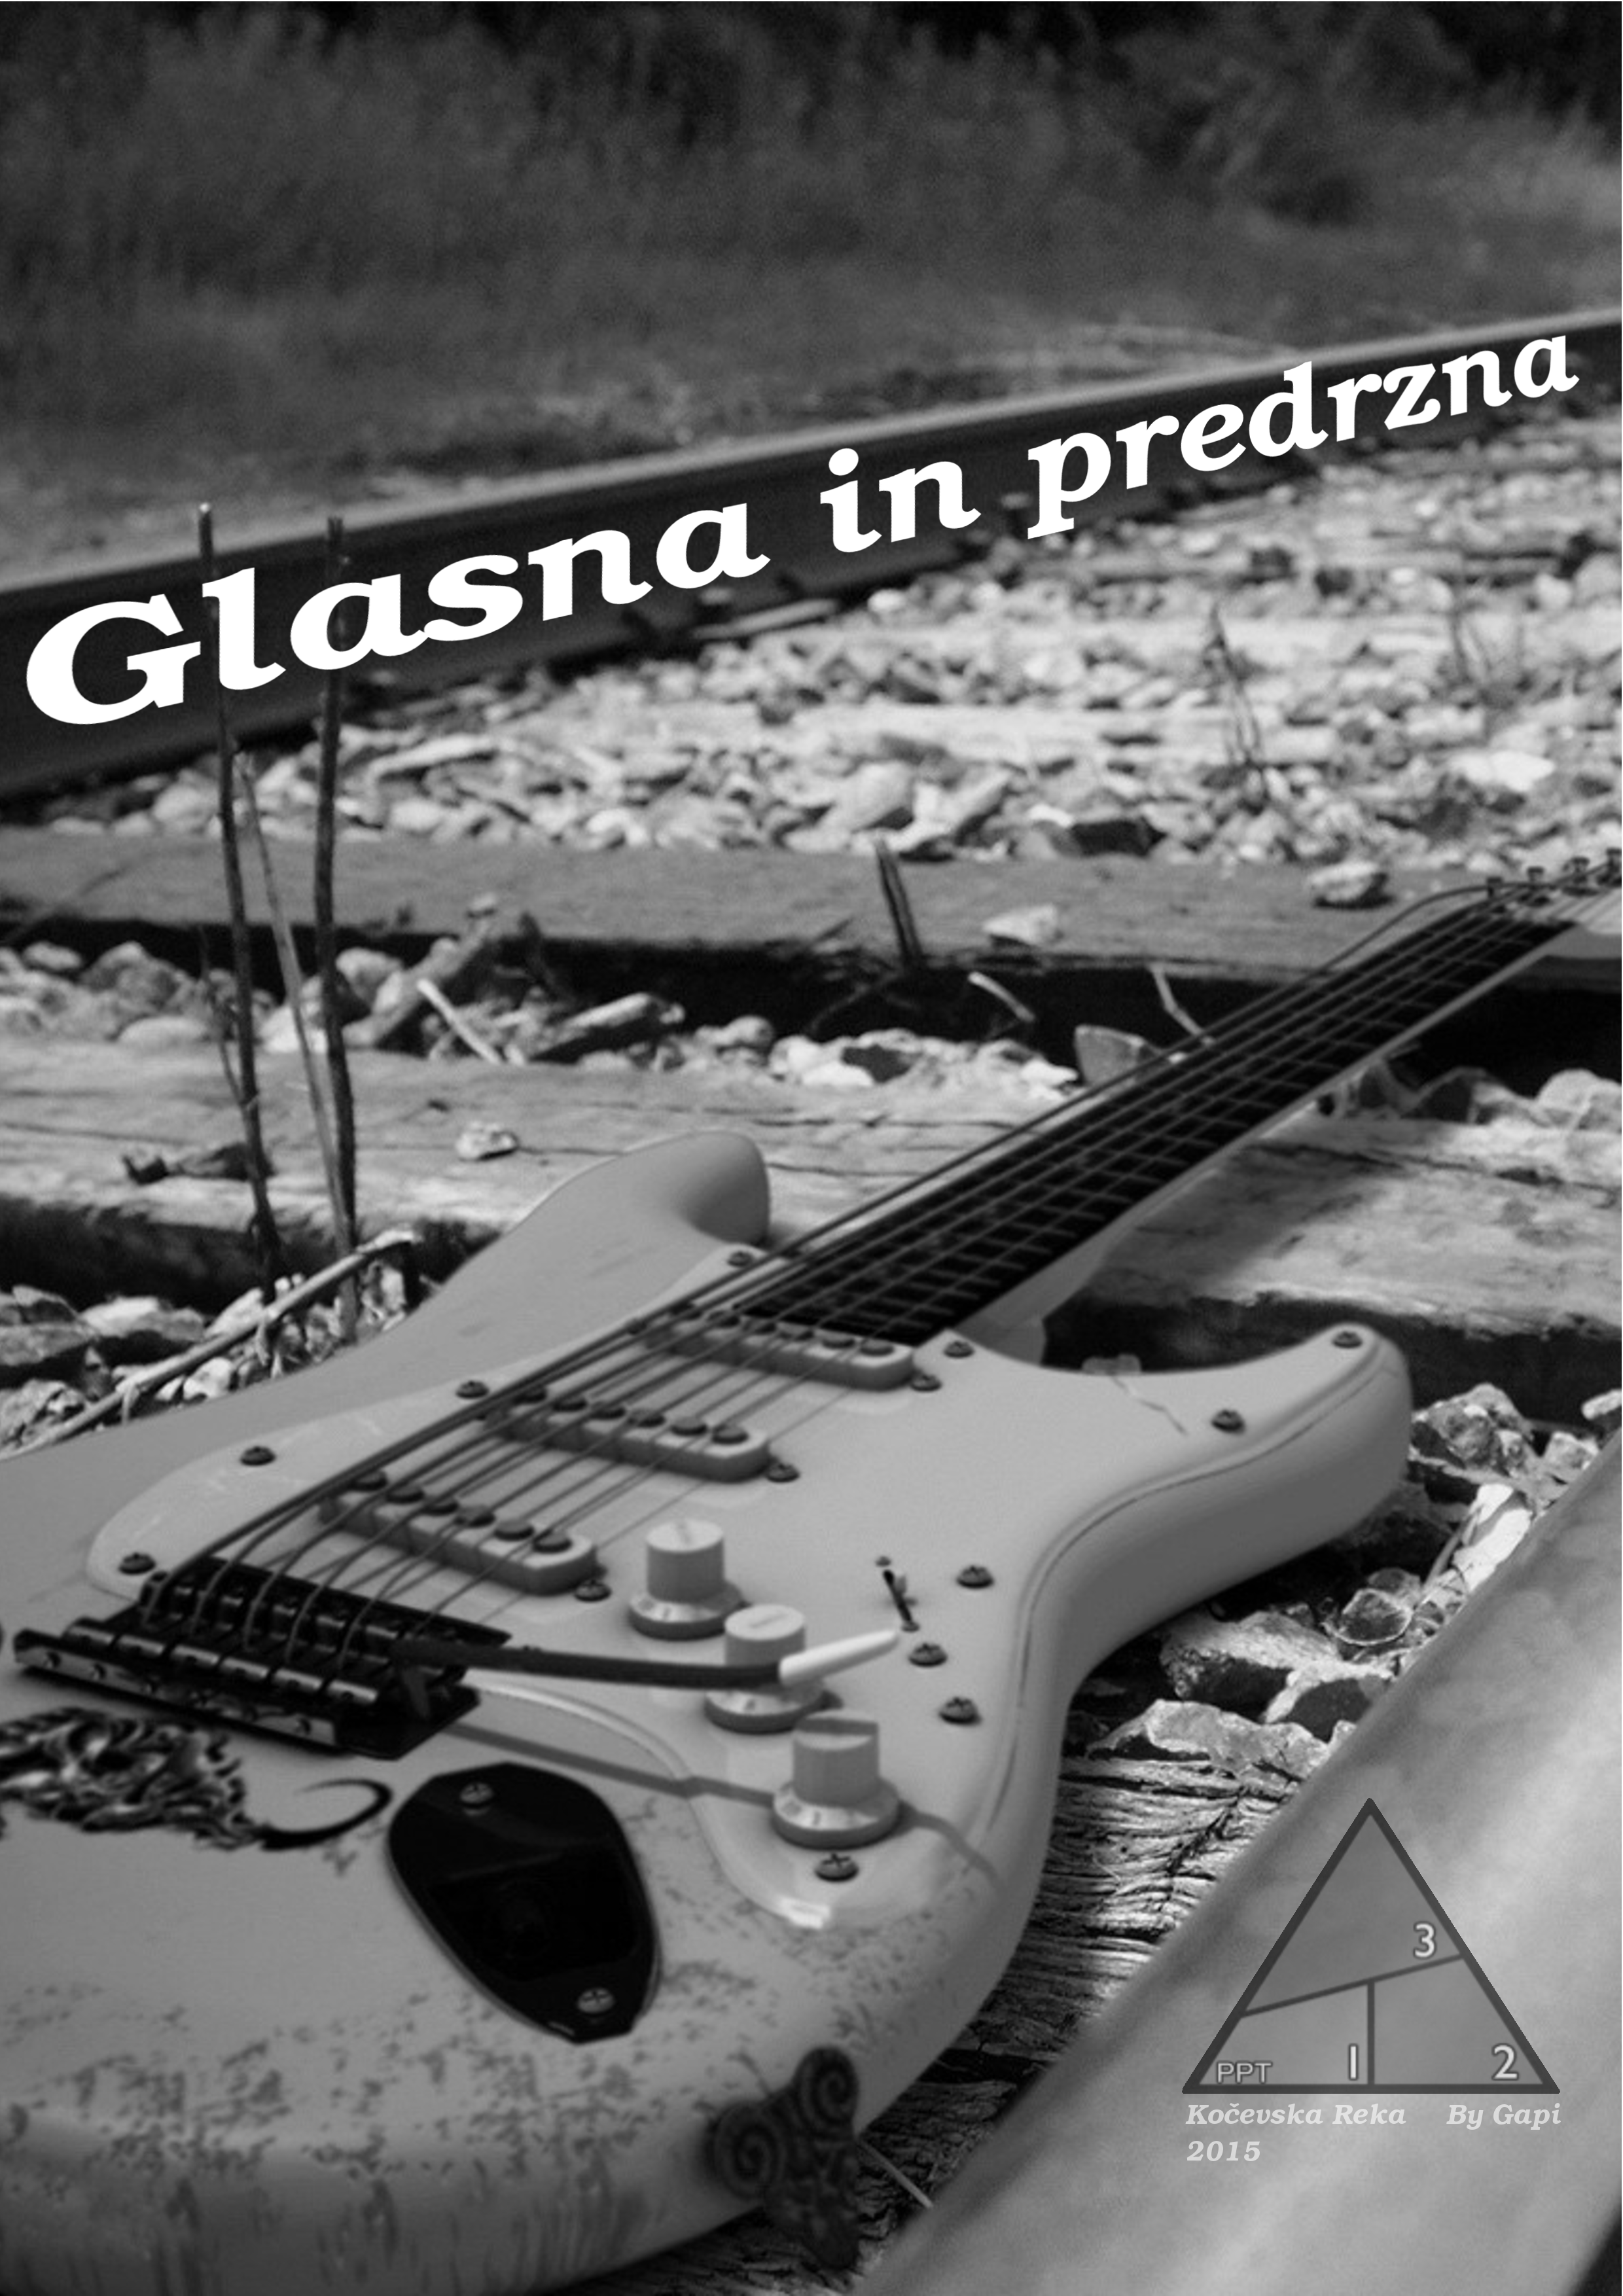
\includegraphics[width=\paperwidth]{img/tpage.png}
\end{textblock*} \
\end{titlepage}
\setlength{\columnseprule}{0.5pt}
\begin{multicols}{2}
\tableofcontents
\end{multicols}
\pagebreak

\setlength{\columnseprule}{0.5pt}
\begin{multicols}{2}
\pagenumbering{arabic}
\section{Akordi}
\begin{guitar}
[A - X02220  Am - X02210]

[B - X13331  Bm - X13321]

[C - X32010  Cm - X35543]  

[D - XX0232  Dm - XX0231] 

[E - 022100  Em - 022000] 

[F - 133211  Fm - 133111]

[G - 320003  Gm - 355333]

[H - X24442  Hm - X24432]


[A7 - X02020  B7 - X13131]

[C7 - X32310  D7 - XX0212]

[E7 - 020100  F7 - 131211]

[G7 - 320001  H7 - X21202]


[Am7 - X02010  Bm7 - X13121]

[Cm7 - X35343  Dm7 - XX0211]

[Em7 - 022030  Fm7 - 131111]

[Gm7 - 353333  Hm7 - X24232]


[C# - X46664  D# - 779997]

[F# - 244322  G# - 466544]


[C#m - X46654  D#m - 779987]

[F#m - 133111  G#m - 466444]


[A6 - X02222  C6 - X055555]

[D6 - X077777 E6 - X099999]


[ASUS2 - X02200]

[ASUS4 - X02230]

[DSUS2 - XX0320] 

[DSUS4 - XX0233]

[ESUS4 - 022200]

[CMAJ7 - X32000]

[FMAJ7 - 103210]

[GMAJ7 - 3X0032]

[DADD4/ADD2 - 554030]

\end{guitar}
\subsection*{Barre akordi}
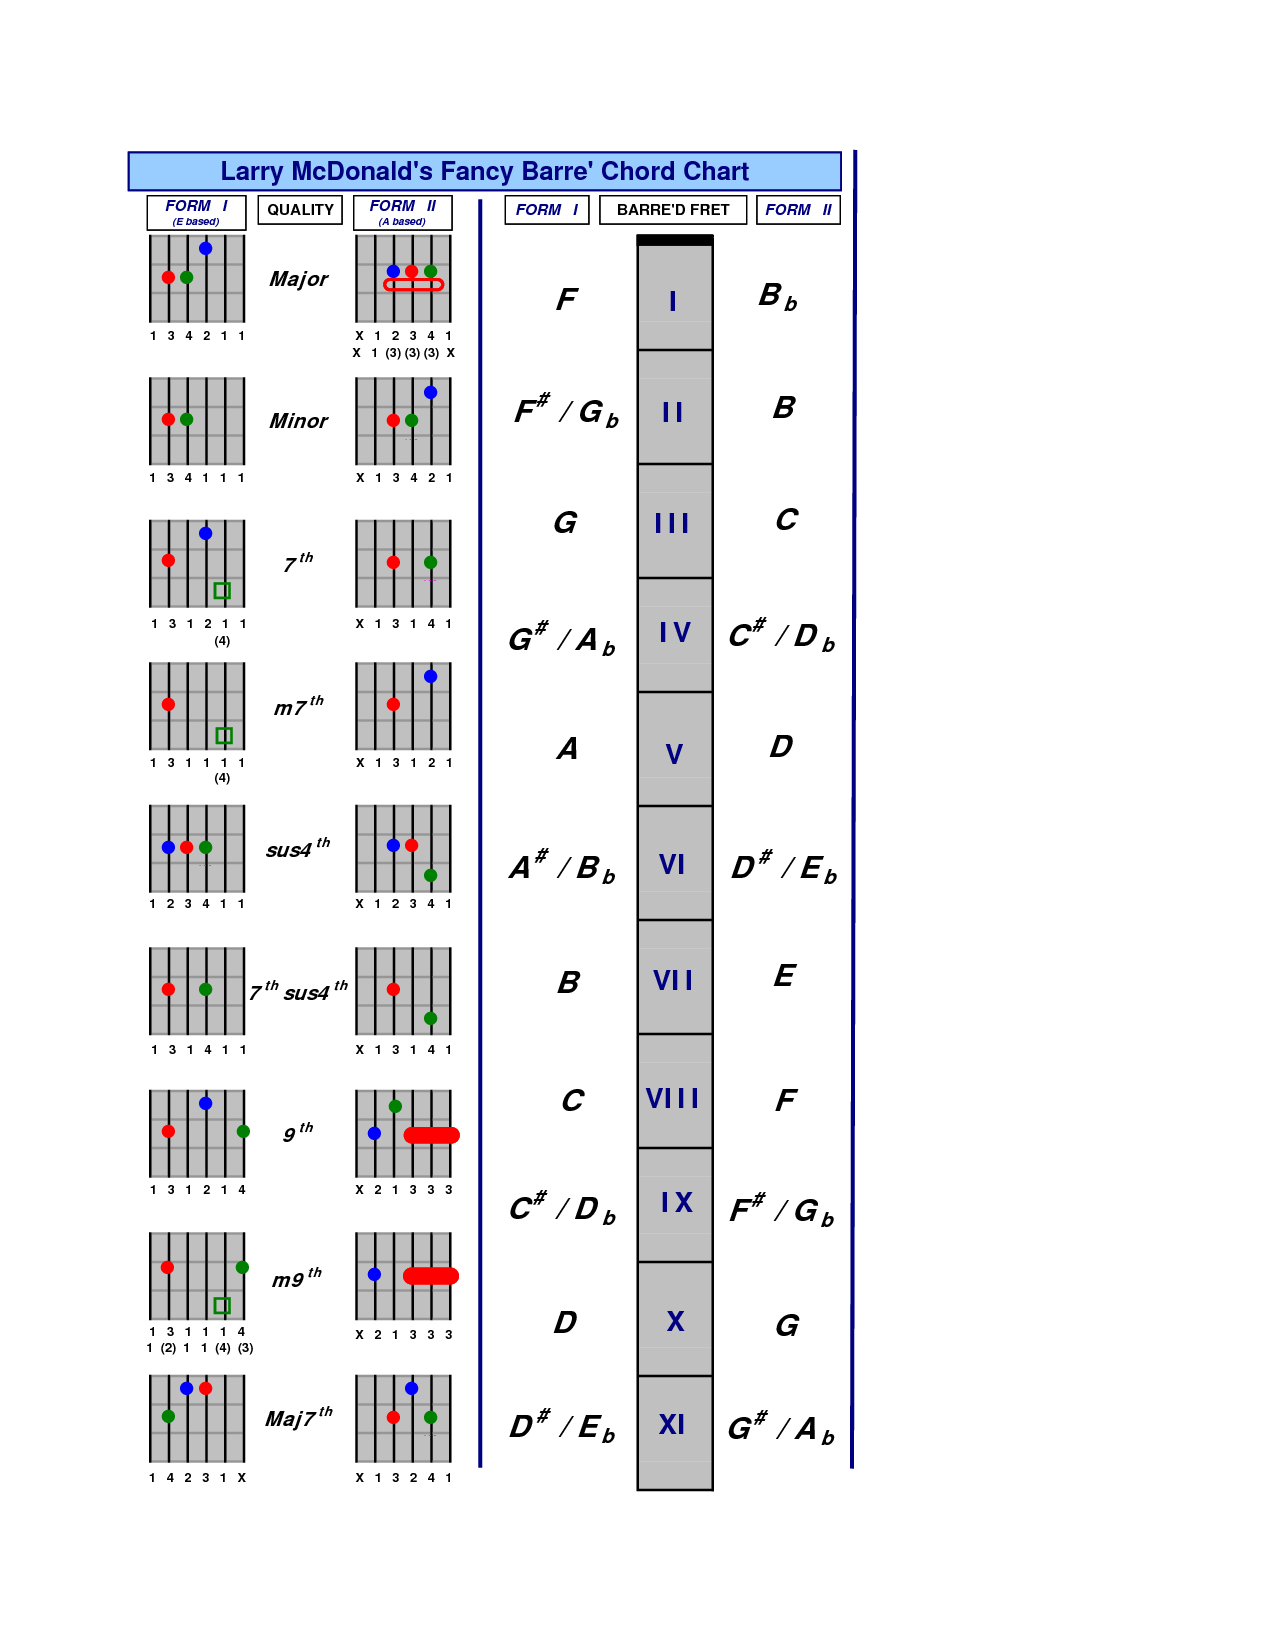
\includegraphics[width=140mm]{img/barre.png}
\clearpage
\section{Gorska roža}
\subsection*{Andrej Šifrer}
\begin{guitar}
[D]Odšel bom tja kjer je daljši dan,
kjer se [G]mestni svet kon[D]ca.
[D]Kjer namesto asfaltnih cest
[A7]vodi le steza. [D]


Hiše razpršene so
kot jata plahih jerebic.
Čas utripa drugače če živiš
v eni od gorskih vasic.


Tisti večer sem žganje pil,
kot ga pije gospodar.
Bog mi v jezik je dal moči
in takrat sem jo spoznal.


Soseda mlada prisedla je
srečal njene sem oči.
Ko smo peli sem jo gledal,
kako se mi smeji. [D7]

  
[G]Gorska roža [D]caka me,
[A7]gorska roža, da [D]vrnem se,
[G]moji Špeli [D]iz planin,
[A7]pod srcem pustil [D]sem spomin.


Brez staršev je, a fantov ni,
ki bi ženili se v gore.
Zjutraj gre v tovarno
saj z majhno kmetijo pač ne gre.


Vzela me je čeprav sem bil
zanjo skoraj še otrok.
Naučila me je piti med,
a jaz sem dal ji svojih 18 let.


Gorska roža...


Od takrat sem pri njej živel,          
na gruntu ob koncu vasi.
Čez dan kitaro sem igral 
in ljubil Špelo vse noči.


Bil opran sem in vedno sit,
jedel kruh sem iz njene peči.
Vstajala je zgodaj, na delavski
avtobus se vedno mudi.


Gorska roža...


Ko zadnja košnja v kozolcu je,
čutiš hladen že objem.
Postajal sem nemiren, 
saj začutil sem jesen. 


Ki pravi:


O dreja poglej okrog,
zdaj postal si del planin.
O dreja jaz se bojim, 
da nekoč te ne izgubim.

\end{guitar}
\section{Ljubljanske ceste}
\subsection*{Aleksander Mežek}
\begin{guitar}
[D]Si že videl s[A]tarca 
[Hm]tam na bližnjem [D]trgu,
[G]v raztrgani o[D]bleki 
pro[A]daja časopis? 
[D]Iz oči ne s[A]ije mu prev[Hm]zetnost 
ne sovr[D]aštvo,
[G]vse kar on i[D]ma,
je k[A]ošček pločni[D]ka. 


Ka[G]ko moreš [D]reči, da [A]sam si [Hm]ti
[A]in sonca zate da več [A7]ni.
[D]Naj te primem [A]pod roko     
in [Hm]peljem po lju[D]bljanskih cestah,
[G]videl boš stva[D]ri, ki [A]te [A7]spreme[D]ne. 


Si že kdaj opazil 
ostarelo ti dekle na cesti? 
Kar na njej visi, 
zamazano je vse. 
Nima časa za klepet, 
kar naprej po mestu blodi, 
njen dom in svet 
je v majhnem kovčku ujet. 


Kako moreš reči... 


In ko mesto ugaša 
v ulični kavarni, 
sam ob črni kavi 
star možak sedi. 
Opazuje svet, 
ki se giblje mimo njega, 
dokler ga natakar 
grobo ne odslovi. 


Kako moreš reči...

\end{guitar}
\section{Ne u tojimi stili}
\subsection*{Ana Pupedan}
\begin{guitar}
[G]Ma ne, nej u tuojmi stili
Pustet me umret na konci bar[D]jače
[C]Ne nej u tuojmi [G]stili.


[G]Ma ženska mene u [D]postlo ma [C]greha [G]ne
[G]Lubezen v rakah [D]unga ku [C]neč ne [G]cuti
[G]Jest sm ti dal lu[D]bezen sm [C]mislu na [G]tebe
[G]In kaj si ti meni [D]dala?
[C]Vinu [G]grenku, [C]Vinu [G]grenku


[G]Ko sm prvič srečal jo je mela krive [D]noge
[D]Ko sm drugič srečal jo so [C]ble ko[G]smate
[G]Maaaa je primem za [D]vime
[D]Ko ga [C]porinem vse [G]mine


Ma ne, Nej U Tuojmi Stili
Pustet me umret na konci barjače
Ne Nej U Tuojmi Stili.


Ma ženska mene u postlo ma greha ne
Lubezen rakahunga ku neč ne čuti
Jest sm ti dal lubezen sm mislu na tebe
In kaj si ti meni dala
Škof vode.


[G]Za vogalom počepnite, eno kilo ga spus[D]tite
In u papir si ga zavite in domov si ga nesite
Da vam bo [D]lepo [C]smr[G]delo

\end{guitar}
\section{Ostani z nami}
\subsection*{Andrej Šifrer, RSK}
\begin{guitar}
[G Em C]        
  
O[D]stani [G]z na[Em]mi,  [C]ostani z [D]nami do [G]jut[Em]ra,  [C]

o[D]stani [G]z na[Em]mi,  [C]vse do [D]belega [G]dne. [Em C D]


[D]Vem, da do[G]voli tvoja [Em]mama [C D]

[D]in je pri[G]kimal tudi [Em]ata, [C D]

[D]pa presl[G]išal stari [Em]deda, [C D]

[D]babica [G]rekla je se[Em]veda, [C D]

[D]ker se [G]strinja zbor [Em]tet, je do[C]volil hišni s[D]vet.[C] 


Ostani z nami... 


Odprli bomo nov sod, 
da bomo vidli kaj je not, 
točajke lepe mlade, 
v čase vlijejo razvade, 
primakni hitro svoj stol  in ne sili domov. 


Ostani z nami... 


Mi bomo pili, mi bomo pili in peli, 
mi bomo pili, dokler grla zdrže. 
    
    
In ko poidejo moči, ko večina obleži, 
v kozarcih se prikaze dno, 
preden petelini zapojo, 
takrat te primem za roko, šepnem ti na uho.


Ostani z mano...


Why don't you stay,
just a little bit longer.
Why don't you stay,
just a little bit more.


Djevojke u ljetnim haljinama volim.
Djevojke u ljetnim haljinama volim.
Volim ih u leđa.
Što mirišu na smolu.
Moj je grad veèeras dobio luku.


Big girls don't cry,
big girls don't cry.
big girls, they don't cry.
They don't cry.


My girl
Six feet high
six feet high
My girl, She doesn't cry.


I said hey, hey baby, U, A
I wanna know if youl'd be my girl. 2x

\end{guitar}
\section{Resničen svet}
\subsection*{Ana Pupedan}
\begin{guitar}
[G]Raje kot gledam te [D]crne oblake
[C]Raje odpravim se v [G]raj na sprehod.
[G]Kupim si liter [D]pravega žganja
In od[C]pravim se v predmestje ne[D]bes.


Opazujem ljudi poznane in tuje,
Ki zavračajo mi moj pogled.
Vzpostavljam tud stke z tistim početjem
Ki mi prej ni bilo všeč.


Panično iščem zavetje rešitev.
Rad našel bi kritje pred nevarnostjo.
Pulim lase si mencam si oči
Nekdo me gleda z radovednost.


Potujem od ene žrtve do druge
Pozorno pošlušam tegobe ljudi
Rad reši bi sebe rešil bi druge
A sploh ne vem če sm živ.


[G]Je to resničen svet ali [A]sanje 
ki jih preveč [D]dobro poznam?


Je to [G]sila peklenskega [A]zla 
ki odpira mi [D]vrata vsa?


Je to spo[G]min iz prejšnjega dela 
živ[A]ljenje ga [D]več ne pozna?


[C]Ali je to le živ[G]ljenje pijanca 
ki ga [D]noče nihče več poznat?


[C]Ali je to le živ[G]ljenje pijanca 
ki ga [D]noče nihče več poznat?


Počasi me spet žganje popušča
počasi se glava bistri
Počasi me spet strah spreletava
saj me kruta resničnost lovi.


Počasi spet vidim na pol manj ljudi
Kot sem videl jih užgan
Vidim tud nekaj ljudi s steklenico
Prazno pa žganju diši


Gledam te črne oblake na nebu
Še bolj so zdaj črni vsi.
Rad videl bi ptico na nebu
Ki ojlčno vejico v krempljih drži


Rad bi tudi da bi sonce me grelo
A tudi sonce zdaj več ne živi
Nimam denarja za še en liter žganja
In to me tudi najbolj skrbi


Je to resničen svet...

\end{guitar}
\section{Romanje}
\subsection*{Andrej Šifrer}
\begin{guitar}

[G]To je mesto, [Hm/F#]ki ne mara tujc[Em]ev
na c[G]estah s[Hm/F#]koraj da ni več ljudi.[Em]

Le f[C]antje s komun[Hm]ale so še b[Am7]udni
s ceste spr[H]ali bodo d[C]an in smet[G]i.
 

Ob desetih so zaprli vse lokale
v mestu je zavladal nočni mir.
Na železniško postajo se odpravim
tam edini točijo še nočni pir.


[G]Kot da tukaj m[Hm/F#]esto še ne sp[Em]i,
k[C]ot da tukaj m[Hm]esto še ž[Am7]ivi
romajo vs[C]i v barkah življenja
nosi jih v[D]eter alkoholnega vrenja
glej noč nam prin[C]aša novega gosta
nekaj boš sp[D]il in z nami odšel
na r[G]oo[Hm/F#]ooooooooooomanj[C]eeeee[D]eee,
r[Em]oooooo[D]oooooooomanj[C]e, [Am F#]

[Hm]na r[Em]ooooo[D]oooooomanj[C]e,
r[Am]oooooooooma[D]aaaaanj[Em]e.


Obraz izdaja, če noči so predolge,
roke izdajo, če težak bil je dan.
V oči upi pa govorijo drugo zgodbo
o vlaku, ki ga čakamo zaman.



\end{guitar}
\section{Siva pot}
\subsection*{Aleksander Mežek}
\begin{guitar}
[G]Skoraj raj si, [Em]ti Gorenjska. 
[D]Sive gore i[C]n zelene r[G]eke. 
Tu življenje skr[Em]iva svoj zaklad. 
[D]Stara si kot sonce, m[C]lajša kot poml[G]ad. 


Siva p[G]ot, vodi [D]me, 
kamor h[Em]oče src[C]e. 
Na Gor[G]enjsko, kjer go[D]re so, 
vodi [C]me siva p[G]ot. 


Le spomini še živijo. 
Zemlja stara, trda neizprosna. 
Rdeča roža v tvojih je laseh, 
nežna mesečina, solza v očeh. 


Siva pot... 


[Em]Ko vstaja j[D]utro slišim p[G]tice iz daljave, 
[C]radio spo[G]minja me na d[D]om tam nekje. 
[Em]In ko se v[F]ozim po be[C]tonskih ma[G]gistralah,
mislim [D]nate le, nate [D7]le... 


Siva pot... 

\end{guitar}
\section{Uspavanka za Evo}
\subsection*{Andrej Šifrer}
\begin{guitar}

Vsaka [G]zvezda na [Em]nebu [Am]zami[D]zi, 
teta [G]Luna pri[Em]kima, [Am]se zasme[D]ji. 
Poga[G]sili [Am]smo v[Hm]se luči, 
da naša [C]Eva lah[D]ko zas[G]pi. 


Vsaka zvezda na nebu zamiži, 
teta Luna prikima, se zasmeji. 
Pogasili smo vse luči, 
da naša Eva lahko zaspi. 


Pa naj z[Em]aspi, naj skrije svoje [D]trudne oči, 
pa naj za[Em]spi, da se malo sr[D]ce umiri 
in naj [G]sanja le o [Am]lepih stvareh. 
Ko [C]sonce zbudi jo, na ustih bo [D]smeh. 


Vsaka zvezda na nebu zamiži, 
Evin kužek zalaja, se poslovi. 
V kraljestvo škratov, sanj in vil 
jo nese sila nevidnih  kril. 


In že leti daleč proč od tega sveta, 
od tega kar ne razume in kar ne pozna, 
saj jo čaka svet drugačen od sanj. 
Kako naj svarim jo, kaj rečem ji v bran? 


[C]Boj se ljudi, ki ne [Am]znajo jokati, 
ne [G]gledajo v oči in ne [D]znajo stisnit’ dlan! 
[C]Boj se množic, ki [Am]mahajo s pestmi, 
šo[G]ferjev s klobuki, [D]nabitih na volan! 


Pa naj zaspi... 


Vsaka zvezda...

\end{guitar}
\section{Vsaka rwža jma trn}
\subsection*{Ana Pupedan}
\begin{guitar}
[C]Uba sva bla sred Paljške gmajne, 
ku se [F]j dejlou dan
[C]Bla sva taku ukep, da [F]blo ni za vrjet
[C]Uuu [F]Uuu, ka[C]ku mraz je [F]blu
[G]Aaaaa, če se [F]spunm me še zdej randa


[C]Vsaka rwža jma [F]trn
[C]Vsaka nouč jma [F]jutru
[C]Vsak kau[G]bojc puje [Am]eno in [F]isto
[C]Vsaka rwža jma [F]trn


Poslušam radio 94, na katermi je resničen svet
DJ Krmpi se zavrti, vsak večjer u Tangoti
Uu Uu, na mwurš taku
Aaaaa, kašna bala


Vsaka rwža jma trn...


Nikul n bom pozabu dnjeva, 
ku smi przadjela hudo bolečino,
Kr ljudje smo u čevljeh 
in ti smi s pjeto stwupla na pauc


Uba sva bla sred Jurške gmajne, 
ku se j dejlou dan
Bla sva taku ukep, da tu nej za verjet
Uu Uu, kaku mraz je blu
Aaaaa, če se spunm me še zdej randa


Vsaka rwža jma trn...

\end{guitar}
\end{multicols}
\clearpage
\clearpage
\null
\vfill
\center

\includegraphics[width=100px]{img/licence.png}

Pesmarica je zaščitena z licenco CC-BY-NC-SA. Vse pesmi so delo in last avtorjev. Morebitne napake in predloge sporočite na pesmarica.info@gmail.com 

Izvorna koda (LaTeX) ter PDF sta dostopna na https://github.com/gztproject/Pesmarica
\end{document}
